\documentclass{article}
\usepackage[utf8]{inputenc}
\usepackage{authblk}
\usepackage{setspace}
\usepackage[margin=1.25in]{geometry}
\usepackage{graphicx}
\usepackage{xcolor}
\usepackage{float}
\graphicspath{ {./figures/} }
\usepackage{amsmath,amssymb,amsfonts}
\usepackage{booktabs}
\usepackage{natbib}
\usepackage{hyperref}
\hypersetup{colorlinks=true, linkcolor=blue, citecolor=blue, urlcolor=blue}

\title{\textbf{The Low-Volatility Anomaly in a Pooled Universe of Large-Cap Equities from Seven Regions}}
\author[1]{SIQuant Research}
\affil[1]{Hypothesis $\times$ Quant}
\date{\today}
\onehalfspacing

\begin{document}
\maketitle

\begin{abstract}
\noindent \textbf{Hypothesis:} $H_0$: the Sharpe ratio of the lowest-volatility quintile does not exceed that of the highest-volatility quintile; $H_1$: it does \\
\textbf{Data:} 108 monthly cross-sections, median 126 stocks from 7 regions, 2017-10 to 2026-09 (formation months) \\
\textbf{Method:} Month-end sort on trailing 252-day volatility, equal-weight quintiles, one-sided stationary-bootstrap test of the Sharpe difference (5,000 draws, block 3) \\
\textbf{Results:} Sharpe 0.84 versus 0.61 (difference 0.23, one-sided $p=0.2887$); mean monthly Q1--Q5 spread -0.89\% ($t=-1.03$). \\
\textbf{Research decision:} \colorbox[rgb]{0.75,0.15,0.15}{\textcolor{white}{\textbf{\,REJECTED\,}}}
\end{abstract}

\section{Design}
The sort variable uses returns up to the month-end of formation and portfolios are held over the following calendar month \citep{baker2011benchmarks,ang2006cross}. Stocks enter only after 252 observed returns, and months without a consecutive successor are discarded rather than interpolated. Returns are in local currency and are not converted, so cross-region currency moves are not part of the test.

\section{Results}
\begin{table}[H]
\centering
\caption{Equal-weight volatility quintiles, monthly rebalanced, local-currency returns}
\begin{tabular}{lcccc}
\toprule
Portfolio & Return & Vol & Sharpe & Max DD \\
\midrule
Q1 low vol & 8.5\% & 10.3\% & 0.84 & -17.0\% \\
Q5 high vol & 15.5\% & 31.9\% & 0.61 & -51.8\% \\
All stocks & 14.4\% & 15.6\% & 0.95 & -20.3\% \\
\bottomrule
\end{tabular}
\end{table}


\begin{figure}[H]
\centering
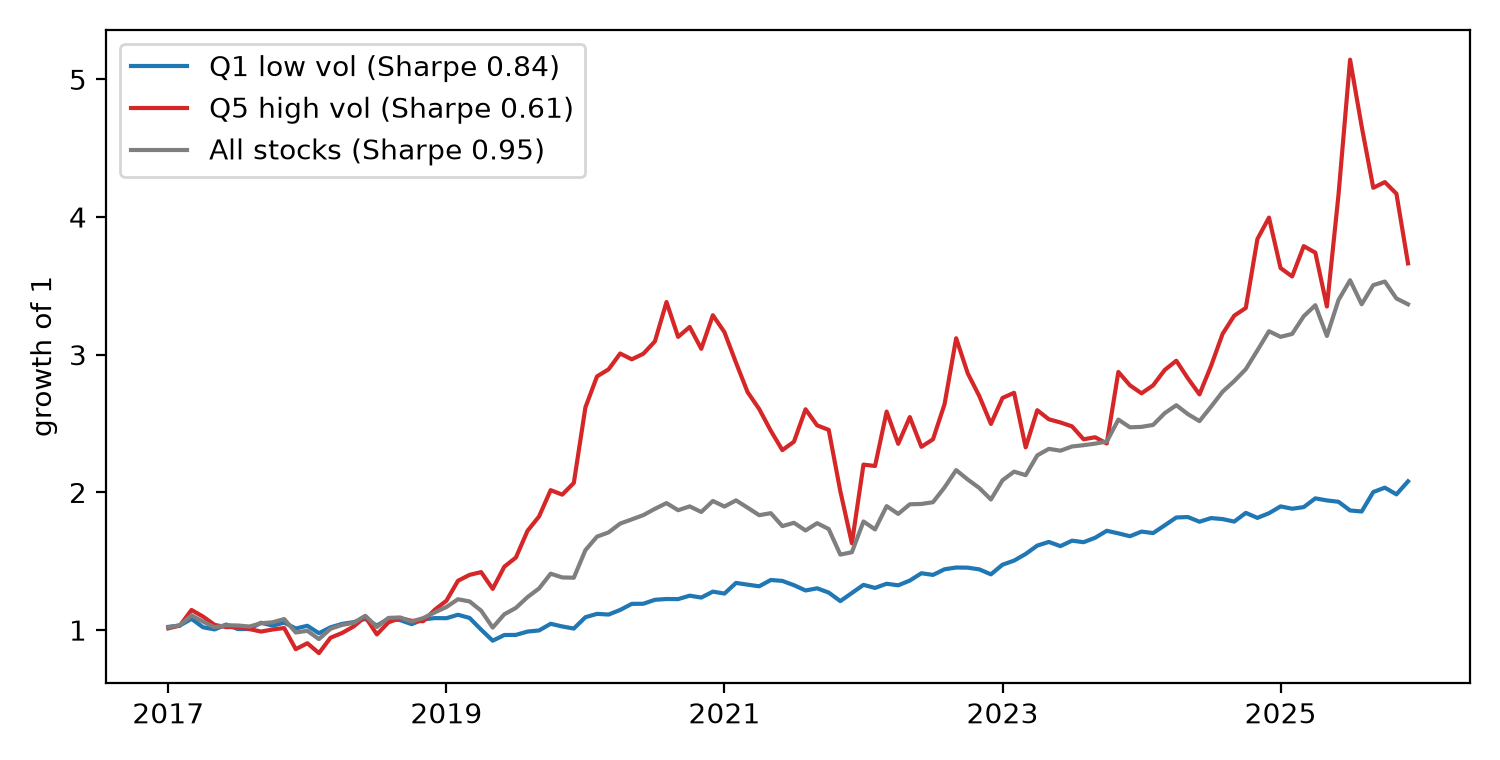
\includegraphics[width=0.8\textwidth]{fig1_low_vol_quintiles.png}
\caption{Growth of one unit in each volatility quintile.}
\end{figure}

\section{Limitations}
The universe is a fixed list of today's large caps, so survivorship bias is present and probably flatters high-volatility winners. There are about 130 stocks, so a quintile holds roughly 25 names; the result need not extend to small caps or to transaction-cost-aware implementations.


\bibliographystyle{plainnat}
\bibliography{references}

\end{document}
